\section{Grundlagen}

Obwohl Dreiecksnetze eine effektive Darstellung bieten, 3D-Modelle darzustellen, beanspruchen diese sehr viel Speicherplatz.
Mithilfe von Brotli-G sollen diese auf der CPU komprimiert, und auf der GPU dekomprimiert werden, sodass diese fertig zur Darstellung sind, ohne viel Bandbreite zu nutzen.
Damit der Weg von Komprimierung zu Darstellung verständlich ist, müssen einige grundlegende Dinge geklärt werden.

In diesem Grundlagenkapitel werden die von Brotli-G genutzen Algorithmen erläutert.
Zusätzlich wird ein Ausblick auf die Grafikpipeline gegeben, und die Stellen betrachtet, bei denen weitere Verbesserungen vorgenommen werden können.
Diese zeigt alle Transformationen, die die Daten eines Dreiecksnetzes von dem GPU Buffer bis zum Bildschirm durchläuft.

\subsection{Brotli Kompressionsstandard}
\label{subsec:brotli}
Brotli-G ist eine Weiterentwicklung des Brotli Kompressionsstand, der von AMD im Jahre 2022 entwickelt und veröffentlicht wurde.
Die AMD Spezifikation bietet parallele Datenverarbeiten nach dem SIMD Prinzip (Kap.~\ref{fig:simd_pattern}) auf Parallelrechnern, wie GPUs und Multithreaded CPUs.
Zum Verständnis des von AMD veröffentlichten Kompressionsmodells ist zunächst ein Blick auf das Original erforderlich. \newline

Brotli ist ein von Google Research entwickelter Kompressionsstandard, der 2013 veröffentlicht wurde.
Er ist darauf ausgelegt, Webinhalte effizienter zu komprimieren als ältere Standards wie Gzip oder Deflate.
BrotliG wurde mit bedacht auf Kompatibilität mit dem offiziellen Brotli entwickelt.
So sollte Brotli auch in der Lage sein, Inhalte, die mit BrotliG komprimiert wurden, zu entschlüsseln.
Zu beachten ist, dass dies nur in diese Richtung funktioniert, und somit Brotli das BrotliG Format nicht dekodieren kann  \cite{BrotliG2022}.

Brotli verwendet eine Kombination vieler Kompressionsalgorithmen, um Inhalte effizient zu komprimieren. 
Brotli's Kern besteht aus einem LZ77 Algorithmus, der in unterschiedlichen Ausführung auch in anderen Kompressionsstandard verwendet wird.
Der LZ77 Algorithmus wird zusätzlich mittels Huffman Codierung optimiert.

\subsection{Parallele Datenverarbeitung}
\label{subsec:flynn}
Michael Flynn unterteilte Rechnerarchitekturen in Kategorien, die Abhängig von der Anzahl der Instruktions- und Datenströme sind. \newline
Die Instruktions- und Datenströme:
\begin{enumerate}
\item[\textit{SI}] (\textbf{S}ingle \textbf{I}nstruction)
\item[\textit{MI}] (\textbf{M}ultiple \textbf{I}nstruction) 
\item[\textit{SD}] (\textbf{S}ingle \textbf{D}ata) 
\item[\textit{MD}] (\textbf{M}ultiple \textbf{D}ata) 
\end{enumerate}
können kombiniert werden. \newline

Dadurch ergeben sich die vier Rechnerarchitekturen \textit{SISD}, \textit{SIMD}, \textit{MISD}, \textit{MIMD}.
\subsubsection*{SISD (Single Instruction, Single Data)}
Die am häufigsten anzutreffene Rechnerarchitektur.
Bekannter unter den Namen Von-Neumann Architektur bearbeitet diese Architektur die auf dem Speicher befindlichen Daten seriell.
Man redet auch von skalaren Operationen auf die Daten.
Rechnerarchitekturen mit SISD sind leicht zu verstehen und die Verarbeitung ist vorhersehbar.
Der Preis dafür ist jedoch eine langsamere Verarbeitungsgeschwindigkeit gegenüber parallelen Architekturen.
\subsubsection*{SIMD (Single Instruction, Multiple Data)}
Um die Geschwindigkeit zu erhöhen, werden Daten, auf denen die selbe Operation ausgeübt wird, parallel verarbeitet.
Das ist bei der Berechnung von Vektoren und Matrizen von Vorteil.
Betrachten wir die Addition zweier Vektoren, so kann der resultierende Vektor berechnet werden, wenn die einzelnen Komponenten der Vektoren addiert werden (siehe Abb.~\ref{fig:simd_pattern}). Der Vertex Shader macht von dieser diesem Konzept Gebrauch, während dieser seine per-Vertex Operationen ausführt \cite{DalCin1996}.
\begin{figure}[htb]
  \centering  
  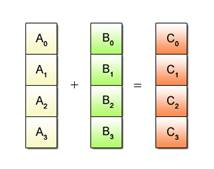
\includegraphics[scale=0.9]{Bilder/Simd_pattern.jpg}
  \caption[SIMD Pattern]{\textbf{Parallele Addition von Daten} Die Abbildung illustriert das SIMD Prinzip anhand eines Beispiels der Vektoraddition. Dabei wird auf verschiedene Daten (die einzelnen Komponenten des Vektors) eine Operation (in diesem Fall eine Addition) ausgeführt.
  Die Abbildung stammt aus \cite{Sony2008}}
  \label{fig:simd_pattern}
\end{figure} 
\subsubsection*{MISD (Multiple Instruction, Single Data)}
Um alle Kombinationen von Daten und Instruktionsströmen zu zeigen wurde auch MISD definiert.
Die Rechnerarchitektur bezieht sich darauf, das auf nur einem Datenpunkt verschiedene Operationen ausgeführt werden.
Für eine lange Zeit war diese Art von Rechnerarchitektur rein theoretisch anzutreffen, da weder 
\subsubsection*{MIMD (Multiple Instruction, Multiple Data)}
Wie auch die SIMD Architektur ist MIMD in Parallelrechnern anzutreffen.
Das Operationsprinzip von MIMD ist die Datenparallelität.
Das Funktionsprinzip von MIMD-Rechnern umfasst die gleichzeitige Ausführung von Anweisungen durch mehrere Prozessoren, die entweder über gemeinsame Variablen oder durch Nachrichten miteinander kommunizieren \cite{DalCin1996}. \newline

GPUs sind Parallelrechner, die auf dem SIMD Prinzip basieren.
Die Many-Core Architektur von GPUs hilft dabei, die richtigen Aufgaben schneller und effizienter auszuführen, als es eine CPU könnte.
Da GPUs Parallelrechner sind, die auf dem SIMD Prinzip bestehen, sind eben jene Aufgaben gut zugeschnitten, die unter den gleichen Bedingungen mehrfach durchgeführt werden müssen.
Wie der Name der \textit{Graphics processing unit} vermuten lässt, wurde diese ursprünglich für die Grafikverarbeitung konzipiert.
Hierbei können die vielen Kerne die selben Operationen auf unterschiedlichen Daten ausführen.
Die auf Durchsatz ausgerichteten Rechner verwenden das Programmiermodel \textit{Single Program Multiple Data (SPMD)}.
Mit diesem Programmiermodell wird ein Programm (Beispielsweise ein HLSL Shader) simultan von mehreren Recheneinheiten ausgeführt.
Zusätzlich dazu werden Threads zur weiteren Effizienzsteigerung in SIMD-Gruppen zusammengefasst \cite{Yilmazer2014}.

TODO später \cite{Jakob2017} \newpage

\subsection{Die traditionelle Rendering Pipeline}
\label{subsec:traditionelle_renderingpipeline}
Um den Nutzen der neu vorgestellten Task- und Mesh-Shader Pipeline zu verstehen, muss zunächst die traditionelle Pipeline dort betrachtet werden, wo sie verbessert werden kann.
Die Rendering Pipeline besteht aus eine Reihe von programmierbaren (Abb.~\ref{fig:traditional_pipeline} grün dargestellt) und fixed-function (Abb.~\ref{fig:traditional_pipeline} türkis dargestellt) Stages.
Dazu kommt, das einige dieser Stages optional sind.
\begin{figure}[htb]
  \centering  
  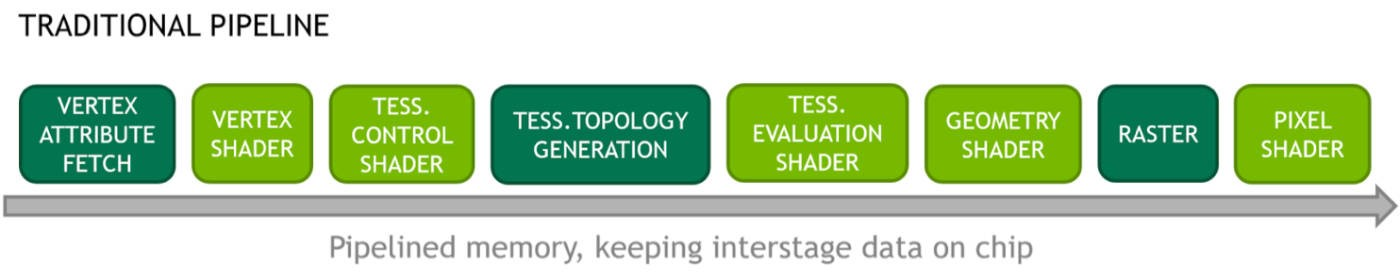
\includegraphics[scale=0.43]{Bilder/traditionelle_pipeline.jpg}
  \caption[traditionelle Rendering Pipeline]{\textbf{traditionelle Rendering Pipeline} \newline Die Abbildung beschreibt den Verlauf durch die einzelnen Shader Stages, die jeder Vertex macht. Entnommen wurde diese aus dem NVidia Blogpost \cite{Kubisch2018}}
  \label{fig:traditional_pipeline}
\end{figure}
\newline
Im GPU Memory angekommen, liest die \textit{Vertex Attribute Fetch} Stage die Vertex Daten aus, und sendet diese an den Vertex Shader.
Die Vertex Daten werden dort in die benötigten Koordinatensysteme transformiert und der optionalen Tessellation Stage weitergegeben, falls diese verwendet wird.
Die Tessellation Stage ist dazu da, Patches von Primitiven in kleinere Primitiven zu unterteilen.
Der optionale Geometry Shader kann dazu verwendet werden, weitere Vertices zu generieren.
Im Rasterizer angekommen, werden Primitiven verarbeitet und daraus Fragmente berechnet, denen der Fragment Shader zum Abschluss ihre Farbe gibt. \newline
Im Folgenden werden die einzelnen Stages nochmal genauer erläutert.

\subsubsection{Vertex Shader}
\label{subsubsec:vertex}
Zunächst wird der vom Entwickler programmierbare Vertex Shader angesteuert.
Dieser ist nicht optional, da alles nachfolgende auf den ausgegebenen Vertices aufbaut.
Hier können Operationen auf einzelnen Vertices ausgeführt werden.
Dafür wird der Vertex Shader für jeden Vertex einzeln aufgerufen.
Hier zeichnet sich das SIMD Modell der GPU aus (Kap~\ref{subsec:flynn}), da der Vertex Shader von mehreren Prozessoren auf unterschiedlichen Vertices zeitgleich operiert.
Die Inputs des Vertex Shaders werden mittels \textit{Vertex Attribute Locations} in den Shader eingebunden.
Der Shader kann dadurch die Positionen, Normalen und Texturkoordinaten von der CPU aufnehmen.
Eine Einschränkung, die dabei aufkommt, ist das Verhältnis von Eingabe und Ausgabe Vertices.
Der Shader erwartet, dass für jeden Eingabe Vertex auch ein Vertex ausgegeben wird.
Die Vertex Position wird für gewöhnlich in den Clip-Space transformiert, und der Pipeline weitergegeben.

\subsubsection{Tessellation Stage}
\label{subsubsec:tesselation}
Die Ausgabe Vertices des Vertex Shaders gelangen anschließend in die optionale Tessellation Stage.
Der generelle use-case ist, einen Patch an Primitiven in wiederum kleinere Primitiven zu verarbeiten. 
Die Tessellation Stage wird in drei Schritte unterteilt.
Darunter ist mit dem \textit{Tessellation Control Shader} (TCS) ein optional programmierbarer Schritt, eine fixed-function mit der \textit{Primitive Generation} und einen programmierbaren \textit{Tessellation Evaluation Shader} (TES).

\subsubsection*{Tessellation Control Shader (TCS)}
Der \textit{Tessellation Control Shader (TCS)} (der wiederum optional ist), ist ein geeigneter Schritt um das \textit{LOD} (Level of Detail) zu berechnen und unter gewissen Voraussetzungen vorab einige Patches zu cullen. 
Ein Patch beschreibt eine Anzahl an Primitiven.
Aus der Subdivision dieses Patches werden weitere Vertices berechnet, die zur Verarbeitung in den nächsten Schritt der Pipeline geschickt werden.
Im TCS wird der Grad der Tessellation, das Spacing zwischen subdivided Punkten und die gewünschte Topologie festgelegt.
Genauer gesagt wird hier gesetzt, wie oft die Primitiven unterteilt werden und welche Form diese am Ende haben sollen (triangle, quad, isolines).

\subsubsection*{Tessellation Topology Generation (TPG)}
Mit der fixed-function stage des Tessellation Schritts werden die Primitiven mittels den im TCS bestimmten Parametern unterteilt.
Die Koordinaten werden anschließend für den Tessellation Evaluation Shader berechnet.
Diese unterteilt die Patches abhängig von den Berechnungen der TCS.

\subsubsection*{Tessellation Evaluation Shader (TES)}
Der \textit{Tessellation Evaluation Shader} hat den einfachsten Job und realisiert lediglich die Arbeit, die von den zwei vorherigen Stages verrichtet wurde.
Die berechneten Koordinaten des TPG werden in dieser Shader Stage interpoliert, um die neuen Vertices zu generieren.
Abschließend werden die aus der Subdivision berechneten Vertices ausgegeben. 
Wenn der optionale TCS nicht genutzt wird, werden default Parameter für den TPG benutzt. \cite{cozzi2012opengl}\cite{Carvalho2022}

\subsubsection{Geometry Shader}
\label{subsubsec:geometry_shader}
Ein weiterer optionaler Schritt in der traditionellen Grafikpipeline ist der \textit{Geometry Shader}.
Er bekommt eine Primitive als Input, und kann keine oder auch mehr Primitiven ausgeben, als er bekommen hat.
Die Fähigkeit zusätzliche Vertices zu generieren ist auch das, was den Geometry Shader besonders macht.
Der Geometry Shader bekommt seinen Input entweder vom TES, oder, wenn die Tessellation Stage keine Verwendung findet, vom Vertex Shader und leitet seine Ausgabe an den Fragment Shader weiter.
Um Bandbreite zwischen CPU und GPU zu sparen, kann ein Geometry Shader ein Dreiecksnetz mit wenigen Dreiecken erweitern und dieses so detaillierter gestalten.
Ähnlich wie bei der Tessellation, die auf \textit{Patches} von Primitiven agiert, verarbeitet der Geometry Shader die Primitiven an sich.

\subsubsection{Pixel Shader}
\label{subsubsec:pixel_shader}
Der Pixel bzw. Fragment Shader ist der letzte programmierbare Schritt der Grafikpipeline.
In diesem werden die transformierten Vertices und Primitiven schlussendlich gezeichnet.
Der Pixel Shader operiert jedoch nicht auf diesen Daten, sondern auf sogenannten \textit{Fragmenten}.
Das bedeutet, bevor der Pixel Shader seinen Input bekommt, müssen Vertices und Primitiven erst durch den Rasterizer.
Nun liegt es am Entwickler, den einzelnen Fragmenten ihre Farbe zu geben.
In einem Modell werden per-Vertex Texturkoordinaten gesetzt, die auf eine Texturemap verweisen.
Im Fragment Shader wird diese Texturemap mittels Sampler interpoliert.
Zusätzlich müssen noch Materialeigenschaften beachtet werden.
Alternativ kann jeder Vertex auch seinen eigenen Farbwert besitzen. \newline

Um der Szene mehr Realismus beizusteuern, kann im Fragment Shader auch ein Lichtmodell implementiert werden.
Beispiele dafür sind \textit{Flat shading}, \textit{Gouraud shading} und \textit{Phong shading}.
Für die Lichtberechnung werden die Oberflächen-Normalen benötigt.
Diese sind entweder in einem Dreiecksnetz gegeben, oder müssen noch berechnet werden.
Ausgabe des Pixel Shaders ist wiederum ein Fragment.

\subsection{Compute Shader}
\label{subsec:compute_shader}
Der Compute Shader gehört nicht zur traditionellen Grafikpipeline, kann darin aber seinen Nutzen finden.
Sie dienen dazu, jede Mögliche Information die gewünscht ist auf der GPU zu berechnen.
Anders als bei den Shader Stages der traditionellen Grafikpipeline (Kap.~\ref{fig:traditional_pipeline}), erwartet der Compute Shader keine definierten Input/Output Daten, wie beispielsweise der Vertex Shader, der als Input und Output einen Vertex erwartet.
Der Compute Shader kann also willkürliche Daten verarbeiten und dabei noch die Parallelisierung der GPU nutzen \cite{Compute24}. \newline

Wie schon gesagt erhält der Compute Shader keine Input Variablen wie beispielsweise der Vertex Shader.
Im Gegensatz zu diesem werden benötigte Daten mittels Buffer und \glqq Shader Ressource Views\grqq\ auf die GPU geladen (in D3D12).
Aber ganz ohne Inputs kommt der Compute Shader nicht aus.
Vor Aufruf des Compute Shaders muss bestimmt werden, mit wie vielen Threads dieser arbeiten soll.
Der Aufruf der Dispatch Methode mittel Grafik API führt dazu, das der aktuell aktive Compute Shader aufgerufen wird.
Die Dispatch Methode nimmt die Anzahl an Threads in drei Dimensionen als Argument.

Dafür gelten jedoch Hardware Limitierungen.
Für die Anzahl der Threads muss gelten
\begin{gather*}
	numThreadsX, numThreads, numThreadsZ \leq 128 \\
	numThreadsX * numThreadsY * numThreadsZ = 1024
\end{gather*}
(Für Compute Shader Version 5\_0)

Um das SIMD Konzept des Compute Shaders zu verstehen sind zwei Variablen elementar wichtig.
SVGroupThreadID und SVGroupID.
TODO

\subsection{Quantisierung von Gleitkommazahlen}
\label{subsec:quantisierung}
Unter Quantisierung versteht man die Reduktion der Genauigkeit von Signalwerten \cite{Strutz2009}.
Sie gehört unter den verlustbehafteten Kompressionsmethoden aus dem Bereich der Datenreduktion.
Im Rahmen dieser Arbeit sollen die Vertex Attribute quantisiert werden.
Die Vertex Attribute bestehen dabei aus einer Position und einer Normalen, die wiederum aus jeweils 3 Gleitkommazahlen bestehen.
Da Gleitkommazahlen im Gegensatz zu ganzen Zahlen aus 3 Komponenten bestehen, muss zunächst geklärt werden, wie diese quantisiert werden können. \newline

Um eine Gleitkommazahl zu konstruieren, benötigt man ein Bit für das Vorzeichen (\textit{Sign Bit}), eine Anzahl an Bits für den Exponenten und Mantisse.
In der Programmiersprache \textit{C++} sind für einer 32 Bit Gleitkommazahl 8 Bit für den Exponenten vorgesehen, während die Mantisse aus 23 Bit besteht.
Der Standard IEEE-754 legt diese Spezifikation für Gleitkommazahlen fest.
Diese kann jedoch von Compiler zu Compiler abweichen \cite{Microsoft2023}.
Die Mantisse stellt eine Zahl zwischen 1,0 und 2,0 dar.
Aus der Mantisse ist der eigentliche Wert einer Gleitkommazahl zu entnehmen.
Der Exponent einer Gleitkommazahl ist für die Skalierung der Mantisse zuständig.
Die Mantisse wird mit dem Exponenten multipliziert, um den absoluten Wert der Gleitkommazahl zu erhalten.
Das Vorzeichenbit entscheidet anschließend, ob die Zahl positiv oder negativ behaftet ist \cite{Widrow_Kollár_2008}. \newline



\subsection{Grundbegriffe der Datenkompression}
\label{subsec:grundbegriffe_datenkompression}
Das Unterkapitel beschäftigt sich mit den Begriffen der Datenkompression, die im Zuge dieser Arbeit Verwendung finden.

\subsubsection*{Informationsgehalt}
Der Informationsgehalt eines Ereignisses beschreibt, wie viele Informationen beim auftreten des benannten Ereignisses gewonnen werden können.
\begin{equation*}
I(s_i) = \log_2 \frac{1}{p_i}
\end{equation*}

\subsubsection*{Entropie}


\subsubsection*{Entscheidungsgehalt}


\subsubsection*{Kompressionsverhältnis}
Aus der Relation der ursprünglichen Daten und den kodierten Daten ergibt sich das Kompressionsverhältnis.
Diese gibt ein gutes Bewertungsmaß, wie gut ein Kompressionsalgorithmus für eine gegebene Quelle funktioniert.
\begin{equation*}
C_R = \frac{\text{ursprüngliche Datenmenge}}{\text{kodierte Datenmenge}}
\end{equation*}

\subsubsection*{Redundanz}
Als Redundanz bezeichnet man zusätzlichen Aufwand, der für die Repräsentation einer Information nicht benötigt wird.
Um die von Brotli-G verwendeten Algorithmen zu verstehen, muss die Quell- und Codierungsredundanz definiert werden.

Die \textit{Quellredundanz} beschreibt die zusätzlichen Informationen einer Quelle (einer Sammlung an Symbolen), die nicht benötigt werden.
Die Quellredundanz ist abhängig von dem Entscheidungsgehalt $\mathit{H_0}$ des Alphabets und der Quellentropie $\mathit{H(X)}$.
\begin{equation*}
R_0 = H_0 - H(x)
\end{equation*}

Unter \textit{Codierungsredundanz} ist die Redundanz zu verstehen, die in den Codewörtern vorherrscht.
Die Codierungsredundanz ist die Differenz zwischen der durchschnittlichen Datenmenge (beispielsweise die mittlere Codewortlänge) und der Entropie.
\begin{equation*}
\Delta R(X) = R - H(x)
\end{equation*}

\cite{Strutz2009}